 \section{Problem Setting} \label{sec:problem-description}
There are several different conveniences a Smart Home system could provide, e.g. being able to dim, or turn off the lights while sitting down.
Some Smart Home systems incorporate cameras, which provides the ability to monitor ones home while being away.
The functionality affects various aspects e.g., security, chores, ease-of-life enhancements, and entertainment.

\subsection{Use Cases}\label{sec:use-cases}
The following use cases explain some of the problems that users of Smart Home solutions may encounter:

\begin{colbox}{Use case: John}
John is enthusiastic about gadgets and new technology. He therefore owns a lot of \sdevs~from various manufacturers, and majority of his electronics are connected to the Internet. John wants to put on a movie, turn on his surround sound, and dim the light. To do so he has to find and open the phone application for the television to turn it on. Next he has to find another application to dim the light. This application is connected to a \hub~that is connected to all of the lights in the living room, which allows him to dim them simultaneous. To fully enjoy the movie, he also wants to turn on his surround sound system. This requires that he finds the Wi-Fi connected controller for the surround system. An illustration of the use case is seen in  \figref{fig:use-case-1}.
\end{colbox}

\begin{figure}[H]
     \center{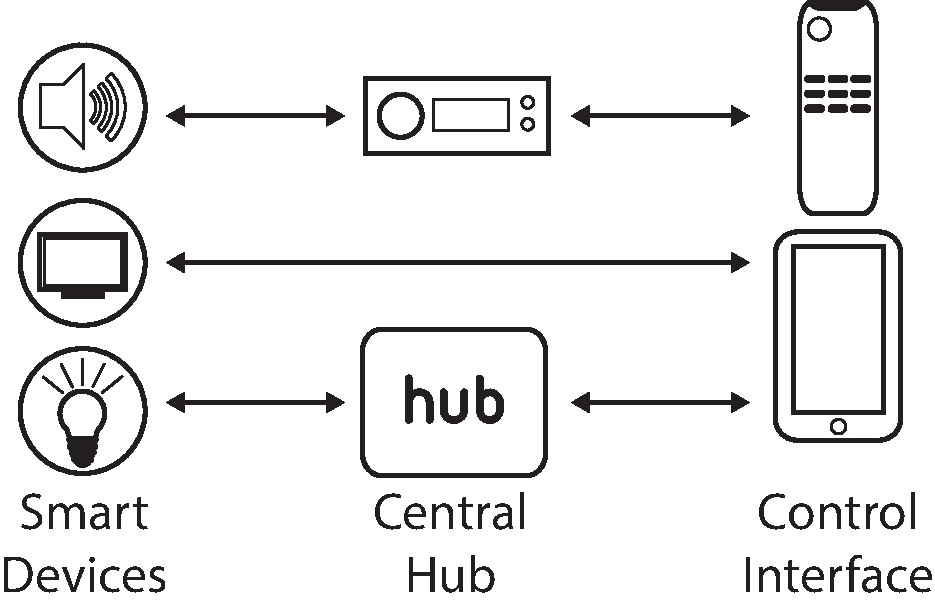
\includegraphics[width=\textwidth -200px]
     {graphics/smarthome-john.pdf}}
     \caption{\label{fig:use-case-1} Illustration of John's use case.}
\end{figure}


\begin{colbox}{Use case: Arthur}
Arthur likes to listen to music when he is at home. He has therefore purchased expensive built-in wireless speakers for every room. The speakers can only be controlled through a \hub~from a \phone. One day Arthur comes home from work and tries to turn on the music, but something is wrong - there is no sound coming from the speakers. After checking both the speakers and the wireless network without results, he discovers that the problem is that the \hub~is broken. He now has to wait for the \hub~to be repaired. This use case is illustrated in \figref{fig:use-case-2}.
0\end{colbox}

\begin{figure}[H]
     \center{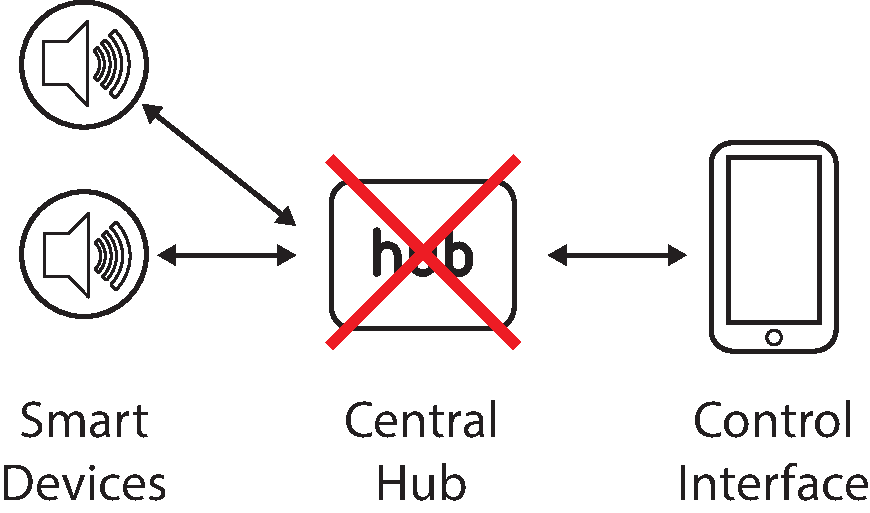
\includegraphics[width=\textwidth -200px]
     {graphics/smarthome-arthur.pdf}}
     \caption{\label{fig:use-case-2} Illustration of Arthur's use case.}
\end{figure}


\begin{colbox}{Use case: Sarah}
Sarah is interested in new technology, and as such she has a Smart Home system. Sarah lives on a farm far away from the city, where she works on the family farm. Unfortunately, Sarah lives in a part of the country where the Internet connection is unstable. Her Smart Home system requires Internet connection to communicate between her devices, where the requests must go through a remote server. This use case is illustrated in \figref{fig:use-case-3}.
\end{colbox}

\begin{figure}[H]
     \center{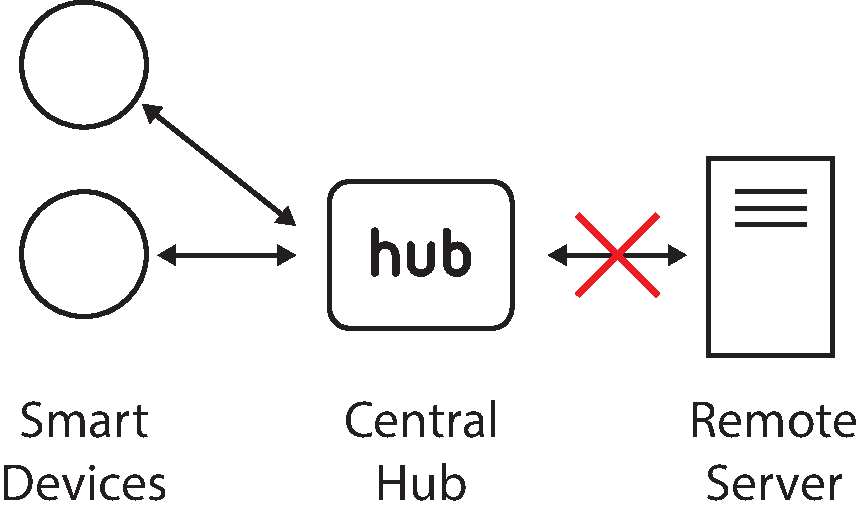
\includegraphics[width=\textwidth -200px]
     {graphics/smarthome-sarah2.pdf}}
     \caption{\label{fig:use-case-3} Illustration of Sarah's use case.}
\end{figure}

\begin{colbox}{Use case: Alice}
Alice lives alone and has a Smart Home system. Usually she is the only one with access to her Smart Home System. One day a new neighbour, Mallory, moved in and asked to borrow Alice Wi-Fi connection for a short period. After some days, the lights and television in Alice's house are turned on at strange times without any interaction from Alice. This use case is illustrated in \figref{fig:use-case-4}.
\end{colbox}

\begin{figure}[H]
     \center{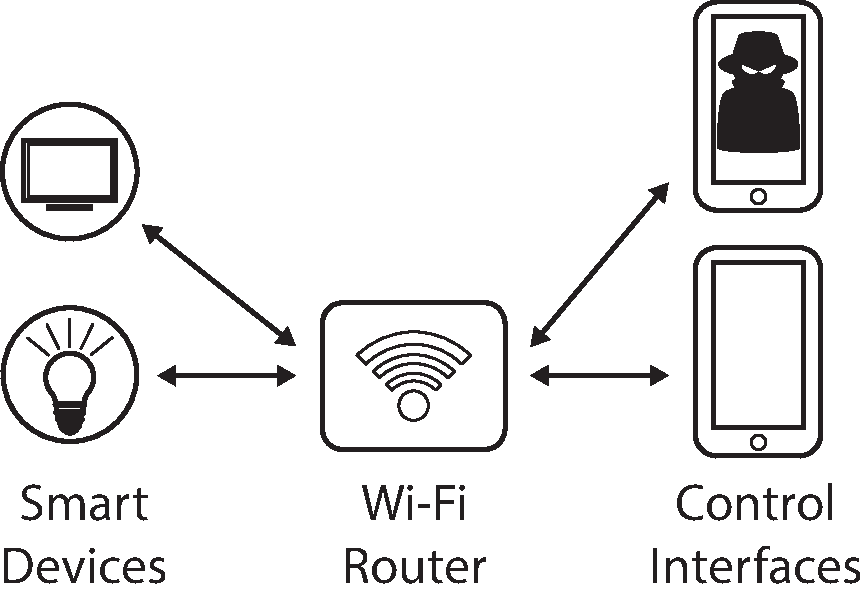
\includegraphics[width=\textwidth -200px]
     {graphics/smarthome-alice.pdf}}
     \caption{\label{fig:use-case-4} Illustration of Alice's use case.}
\end{figure}


These use cases are some of the possible problems that Smart Home owners could have. The four Smart Homes in the use cases suffers from the following issues: no interoperability between manufacturers, centralised around a \hub, requires constant access to remote server, and no user authentication. These problems serve as a base for the further analysis and are referred to through the rest of the report.

\subsection{Smart Home Features} \label{sec:smart-home-features}
When developing a Smart Home system, there are various important aspects to consider. A Smart Home solution should attempt to solve some of the problems occurring in the use cases. Along with the problems found, problems like security, stability, and user-friendliness are also important to consider. The following section are the desired and important properties based on our understanding of the perfect Smart Home system. 

\subsubsection{Stability}
There are two aspects of stability to consider; hardware stability and software stability. \Sdevs~have several external influences which can have unwanted effect on their performance, none of which is preventable with software. The \sdevs~can have an unstable connection to either Wi-Fi or the \hub, they will shut down in case of blackout, and the \hub~can break down. 

Besides the hardware issues, there are also several things that can go wrong on a software level. If the system is not using a \hub~but rather relies on the \phones~being able to connect directly to the \sdevs, a mismatch between the \phones~could occur. Another software instability was found by Raul Rojas. One evening he came home and none of his \sdevs~were working. It turned out that one of his light bulbs had burst and kept reporting it to \hub. This resulted in the light bulb doing a DoS attack on the \hub, which effectively shut down the entire Smart Home~\citep{self-dos-smart-house}.


\subsubsection{Security}
Security is an important aspects to consider. A Smart Home should be secure so that only authorised people can access the Smart Home system. There should also be different levels of access; owners should be able to control the entire system, while guests should only have access rights to the non-sensitive \sdevs. Accessing \sdevs~in a house could potentially expose sensitive data and surveillance media.

Regarding security there are different forms that must be considered. In this project the focus will be on confidentiality, authenticity, and integrity.
\begin{description}
\item[Confidentiality] prevents sensitive information from reaching the wrong people and allowing the right people to access the information.
\item[Authenticity] security of access to devices from people on the same network. Only authorised people should be able to access devices.
\item[Integrity] concerns with keeping the data intact when sent over the network. The data should not be changed by unauthorised people. 
\end{description} 

\subsubsection{Usability}
Setting up a complete Smart Home system can get technical. Ensuring user-friendliness could help expand the market, and improve the user experience. A well designed user interface, or preferred OS compatibility, could also be the deciding factor when choosing the right Smart Home system. This user-friendliness includes both setting up and using the system.

\subsubsection{Interoperability}
Interoperability refers to the ease of connecting additional \sdevs~to the Smart Home system. This is not restricted to \sdevs~from the same manufacturer. As \sdevs~are developed by many different manufacturers it is important to introduce interoperability, a higher level of interoperability could allow easy setup of new \sdevs.

\subsubsection{Feature Contradiction}
These features are all important properties to consider for a Smart Home solution. However it might not be possible to have a high degree of all of these properties as some of them might conflict. Security is, arguably, an important aspect - as no one wants their sensitive data compromised or unauthorised access to their home. This, however, may hurt the usability of the system as it requires management of different access rights.

There are also potential issues with interoperability. It is desirable to be able to connect to any \sdevs, but some devices could possibly have security flaws or other unwanted properties that could both compromise the security and stability of the system.

The stability property in general is intricate. There are multiple areas with potential instability, such as a communicating hub, a Wi-Fi hotspot or the outgoing Internet connection. Attempting to solve these stability issues by cutting corners, changing, or removing some of the precarious spots could potentially give issues regarding the other properties, for instance security or interoperability. 